\documentclass[12pt]{article}
\input{bayesuvius.sty}
\begin{document}

\begin{figure}[h!]\centering
\begin{minipage}{.5\linewidth}
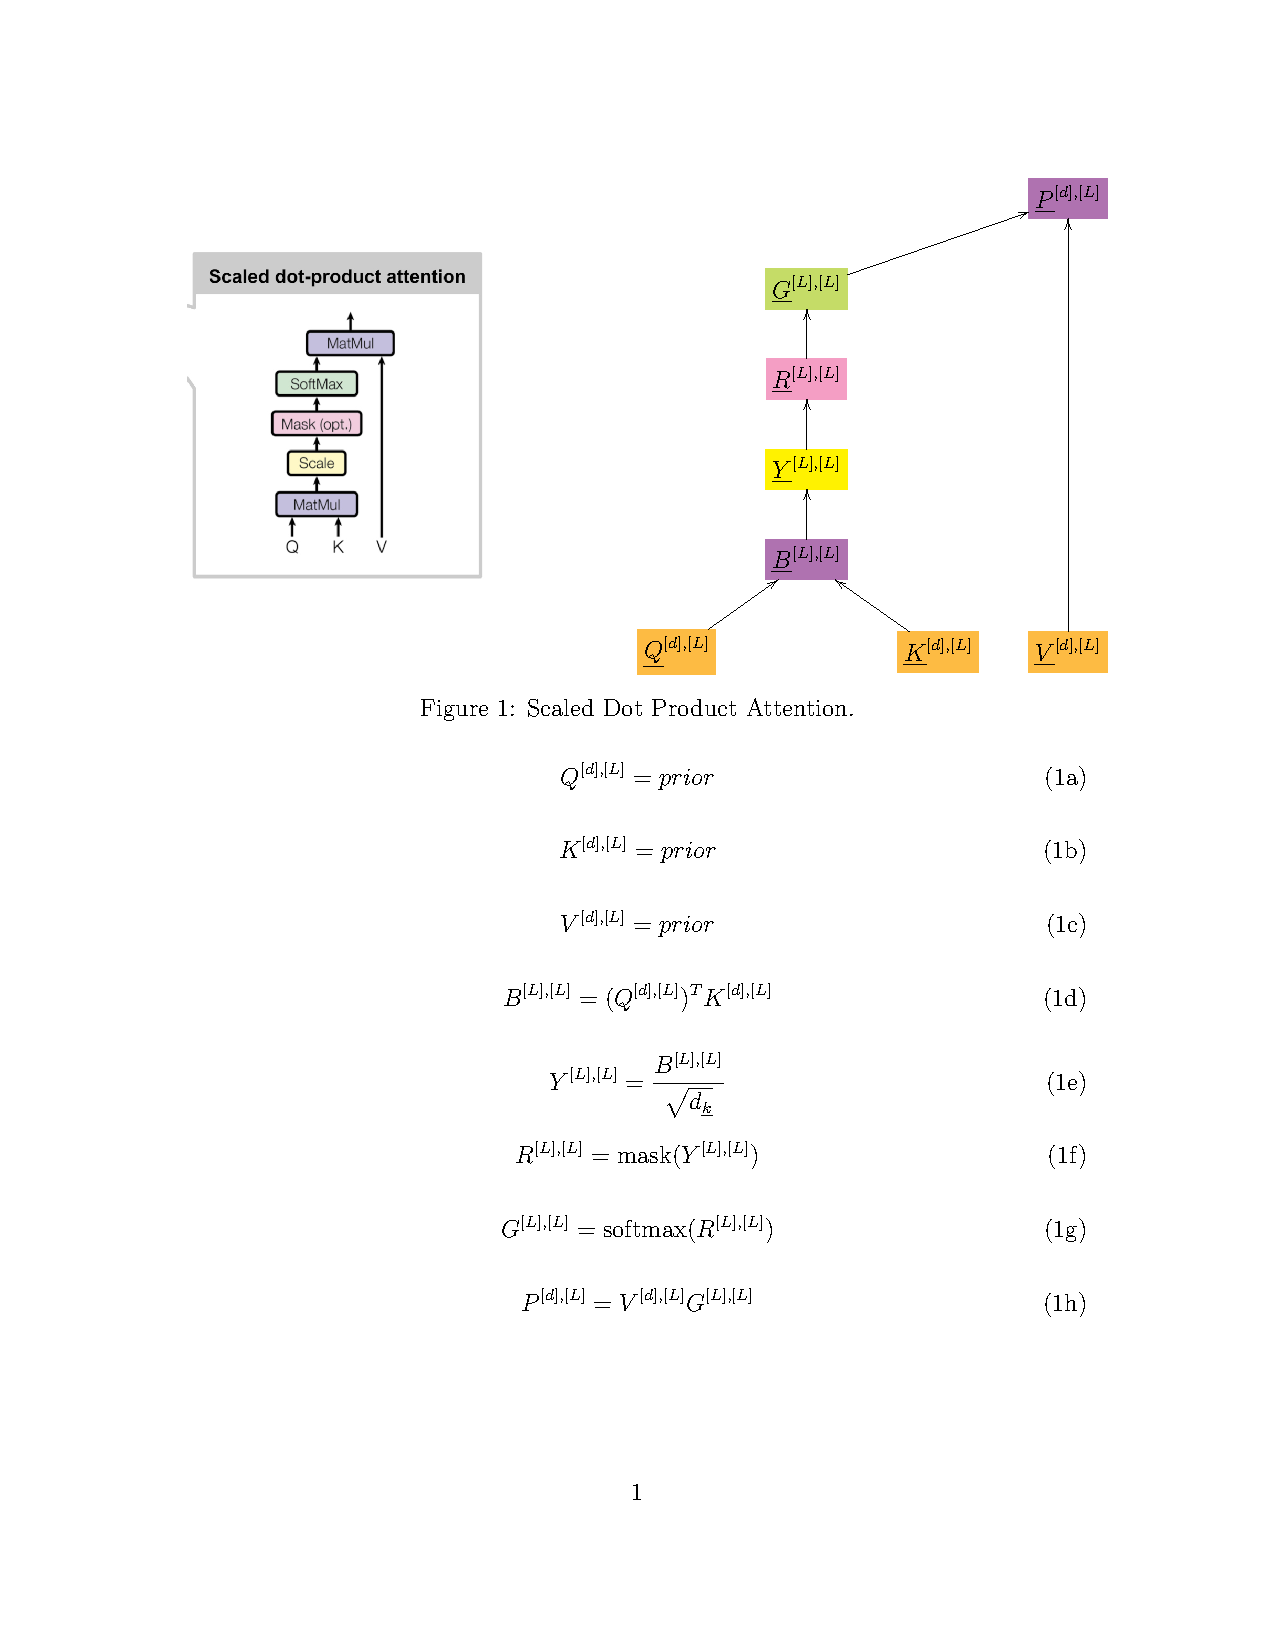
\includegraphics[width=2in]{scaled-dot-prod-att.jpg}
\end{minipage}%blank lines between minispaces breaks this
\begin{minipage}{.5\linewidth}
$$\xymatrix{
&&&*+[F*:Orchid]{\underline{P}^{[d], [L]}}
\\
&*+[F*:SpringGreen]{\underline{G}^{[L], [L]}}\ar[urr]&&
\\
&*+[F*:Lavender]{\underline{R}^{[L], [L]}}\ar[u]&&
\\
&*+[F*:yellow]{\underline{Y}^{[L],[L]}}\ar[u]&&
\\
&*+[F*:Orchid]{\underline{B}^{[L], [L]}}\ar[u]&&
\\
*+[F*:Dandelion]{\underline{Q}^{[d],[L]}}\ar[ur]&&*+[F*:Dandelion]{\underline{K}^{[d],[L]}}\ar[ul]&*+[F*:Dandelion]{\underline{V}^{[d],[L]}}\ar[uuuuu]
}$$
\end{minipage}
\caption{Scaled Dot Product Attention.}
\label{fig-texnn-for-scaled-dot-prod-att}
\end{figure}\begin{subequations}
\begin{equation}
Q^{[d],[L]} = prior
\label{eq-Q-fun-scaled-dot-prod-att}
\end{equation}

\begin{equation}
K^{[d],[L]} = prior
\label{eq-K-fun-scaled-dot-prod-att}
\end{equation}

\begin{equation}
V^{[d],[L]} = prior
\label{eq-V-fun-scaled-dot-prod-att}
\end{equation}

\begin{equation}
B^{[L], [L]} = (Q^{[d],[L]})^T K^{[d],[L]}
\label{eq-B-fun-scaled-dot-prod-att}
\end{equation}

\begin{equation}
Y^{[L],[L]} = \frac{B^{[L], [L]}}{\sqrt{d_\rvk}}
\label{eq-Y-fun-scaled-dot-prod-att}
\end{equation}

\begin{equation}
R^{[L], [L]} = {\rm mask}(Y^{[L],[L]})
\label{eq-R-fun-scaled-dot-prod-att}
\end{equation}

\begin{equation}
G^{[L], [L]} = {\rm softmax}(R^{[L], [L]})
\label{eq-G-fun-scaled-dot-prod-att}
\end{equation}

\begin{equation}
P^{[d], [L]} = V^{[d],[L]}G^{[L], [L]}
\label{eq-P-fun-scaled-dot-prod-att}
\end{equation}

\end{subequations}


\end{document}  
